\hsection{Variable Types and Type Hints}%
\label{sec:variableTypesAndTypeHints}%
%
\hsection{Variable Types}%
\gitLoadAndExecPython{variables:types}{}{variables}{variable_types.py}{}%
\listingPythonAndOutput{variables:types}{%
An example of the types of variables.}{}%
%
A variable is basically a name pointing to an object.
Each object has a type and we already learned about several of these datatypes in \cref{sec:simplyDataTypesAndOperations}.
We can obtain the type of an object stored in variable \pythonil{var} by invoking \pythonil{type(var)}\pythonIdx{type}.
\Cref{lst:variables:types} shows a program that does just that and the output of that program is given in \cref{lst:variables:types}.
It is obvious that the type of a variable that holds an integer value is \pythonilIdx{int}, the type of a variable that holds a floating point number is \pythonilIdx{float}, and so on.
There really is not much to say about that.%
\endhsection%
%
\hsection{Types and Confusion}%
\label{sec:typesAndConfusion}%
%
\gitLoadAndExecPython{variables:types_wrong}{}{variables}{variable_types_wrong.py}{}%
\listingPythonAndOutput{variables:types_wrong}{%
An example of the confusing variable types.}{}%
%
Well, actually, there is.
You see, when you declare a variable in a language like \pgls{C}, you have to specify its \emph{type}.
You are then permitted to only assign values that have exactly this type to the variable.
In \python, you do not need to specify a type and you can assign whatever you want to a variable.
This has the advantage that the code is shorter (because you do not need to write the type), looks more elegant, and programming becomes easier.
At first glance.
However, there are also problems.
Let's take a look at \cref{lst:variables:types_wrong}.
We declare a variable named \pythonil{int_var} and store the integer~\pythonil{8} in it.
Then we update \pythonil{int_var} by computing \pythonil{int_var = int_var / 3}.
Back in \cref{sec:int}, you learned that the \pythonilIdx{//} operator performs an integer division with an \pythonil{int} result, whereas the division using the \pythonilIdx{/} operator always returns a \pythonil{float}.
This means that our variable \pythonil{int_var} now contains a \pythonil{float}, which is also visible in the output in \cref{exec:variables:types_wrong}.

From the perspective of \python, this is totally fine.
The program executes and the output appears without error.
However, from the perspective of programming, \cref{lst:variables:types_wrong} is \emph{wrong}.
Imagine that this was not just some random example without meaning.
Imagine that this was a part of a really useful program.
Imagine that you got this program from some source and try to understand it.
If you read this program, then you find that a variable named \pythonil{int_var} contains a \pythonil{float}.
This is not forbidden, but when reading the code, it must strike you as odd.

Indeed, there are at least two possible explanations for this:
On the one hand, maybe, the original author of this code mistakenly mixed up the \pythonilIdx{/} operator for the \pythonilIdx{//} (see \cref{bp:intDivision}).
Maybe they wanted to do an integer division and accidentally did a floating point division.
Depending on what the code later on (in our imaginary larger program) does, it could be very hard to find such an error.

On the other hand, maybe, the author fully well wanted to do a floating point division and expected a \pythonil{float} to be stored in \pythonil{int_var}, but chose a misleading name.
Choosing this name, however, can be very dangerous:
What if another programmer continues to work on this code and, based on the variable's name, expects it to contain an \pythonil{int} whereas it actually contains a \pythonil{float}.
This could again lead to all sorts of strange errors later on in her code.

\bestPractice{codeClarity}{The names we use in program code should clearly reflect our intentions.}

If the programmer followed \cref{bp:codeClarity}, then the code would clearly contain a bug, namely a mix-up between the \pythonilIdx{/} operator for the \pythonilIdx{//}.
Regardless of what is true, you will certainly agree that something is wrong with this program.
And most certainly, it was just a small oversight, maybe even just a typo.
Unfortunately, since you are not the author of the program, you do not know what is wrong.
This code will cause some problem down the line.
Many such problems exist in many software projects and they indeed are hard to find~\cite{KCVM2022AESOTRDIPP}.
So here, the lenience of \python\ of allowing us to not specify types comes back to bite us.

Everyone of us makes such mistakes.
It is impossible to completely avoid them.
Luckily, there are two things that we can do to prevent such situations from passing our \inQuotes{quality control}:%
%
\begin{enumerate}%
%
\item Use static type checking tools to find such potential errors in our code.%
%
\item Use \pglspl{typeHint} to annotate variables with their types to \emph{a)}~make our intention clearer and \emph{b)}~support type checking tools.%
%
\end{enumerate}%
%
And if you are in one of my classes, you better do both.
And now we will learn how to do that.%
\endhsection%
%
%
\hsection{Static Type Checking}%
%
\begin{figure}%
\centering%
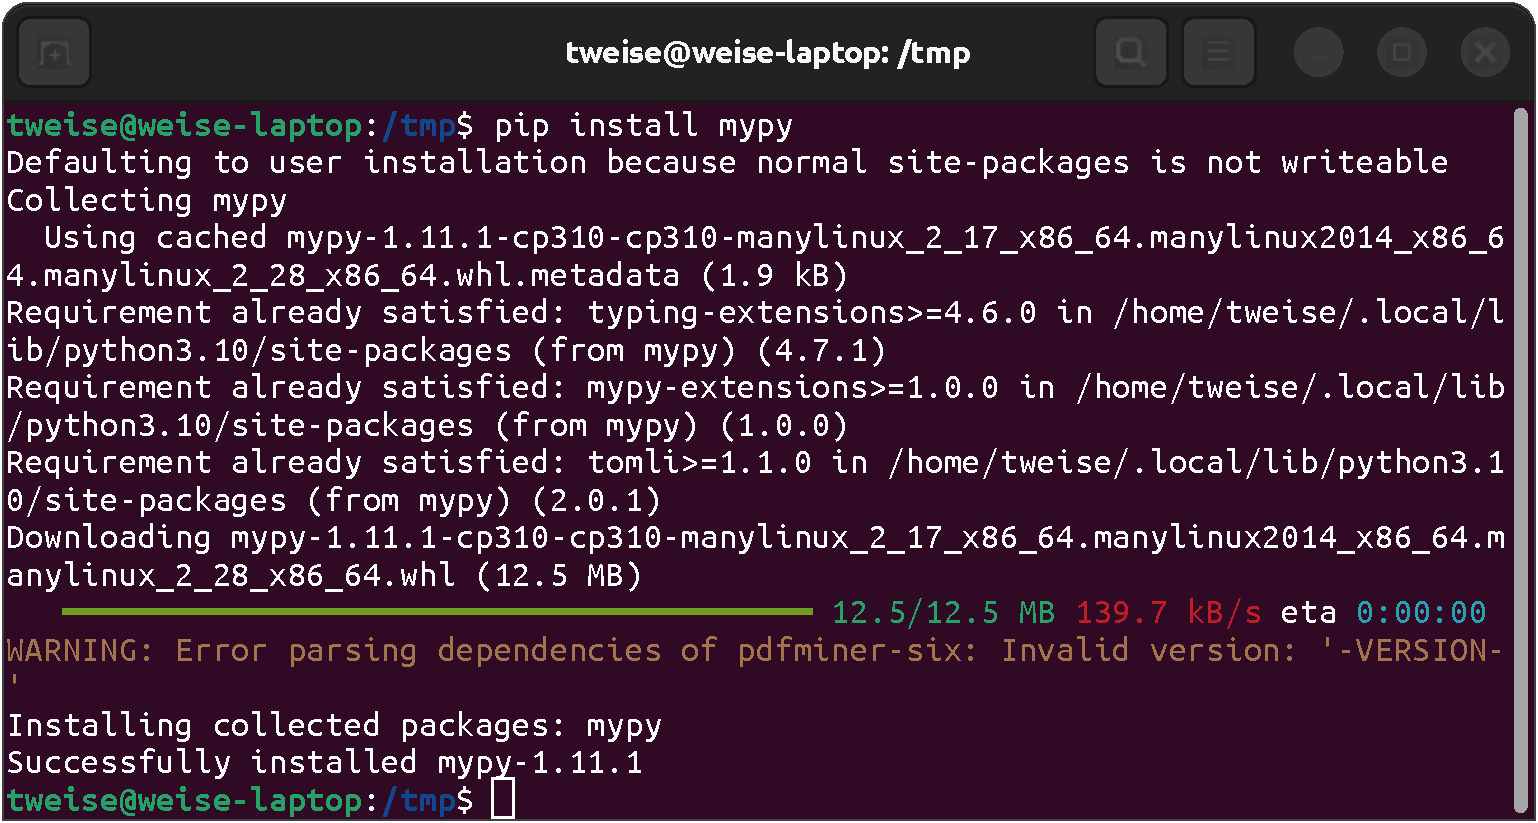
\includegraphics[width=0.7\linewidth]{\currentDir/pipInstallMypy}%
\caption{Installing \mypy\ in a \ubuntu\ \pgls{terminal} via \pip~(see \cref{sec:pipAndVenv} for a discussion of how packages can be installed).}%
\label{fig:pipInstallMypy}%
\end{figure}%
%
\gitExec{exec:variables:variable_types_wrong:mypy}{\programmingWithPythonCodeRepo}{.}{_scripts_/mypy.sh variables variable_types_wrong.py}%
\listingToolOutput{variables:variable_types_wrong:mypy}{%
The results of static type checking with \mypy\ of the program \textil{variable_types_wrong.py} given in \cref{lst:variables:types_wrong}. %
(This is actually output generated by the script~\cref{lst:bash:mypy} on \cpageref{lst:bash:mypy}.)}%
%
\gitExec{exec:variables:variable_types:mypy}{\programmingWithPythonCodeRepo}{.}{_scripts_/mypy.sh variables variable_types.py}%
\listingToolOutput{variables:variable_types:mypy}{%
The results of static type checking with \mypy\ of the program \textil{variable_types.py} given in \cref{lst:variables:types}. %
(This is actually output generated by the script~\cref{lst:bash:mypy} on \cpageref{lst:bash:mypy}.)}%
%
A first step to avoiding any type-related errors in programs is, ofcourse, careful programming.
The second step is to use tools that check whether your program code contains ambiguities or errors.
In languages like \pgls{C}, the compiler will take care of that for you.

In \python, which allows for dynamic typing and is an interpreted language, we will use a tool like \mypy~\cite{LLHSVRZSJYYMC2024MOSTFP}.
You can install this tool by opening a terminal.
Under \ubuntu, you therefore press \ubuntuTerminal, and under \microsoftWindows, you \windowsTerminal.
Then type in \bashil{pip install mypy}\pythonIdx{Mypy}\pythonIdx{pip} and hit \keys{\enter}.
The \mypy\ tool will be installed as illustrated in \cref{fig:pipInstallMypy}.

We can now apply the tool to the program from \cref{lst:variables:types_wrong}.
All we have to do is invoke it in the terminal, giving the program to be checked as argument as well as some additional parameters.
In \cref{exec:variables:variable_types_wrong:mypy}, we invoke \bashil{mypy variable_types_wrong.py --no-strict-optional --check-untyped-defs}, where \textil{variable_types_wrong.py} is the (very fitting) name of the program to check.
Indeed, \mypy\ tells us that something dodgy is going on in the fourth line of that program, i.e., \pythonil{int_var = int_var / 3}.
It will fail with an \pgls{exitCode} of~\bashil{1}.
Programs usually return~\bashil{0} as \pgls{exitCode} if everything went well and some non-zero value if something went wrong.
And something went wrong, because \mypy\ found the error.%
%
\usefulTool{mypy}{%
\mypy~\cite{LLHSVRZSJYYMC2024MOSTFP} is a static type checking tool for \python. %
This tool can warn you if you, e.g., assign values to a variable that have a different type than the values previously stored in the variable, which often indicates a potential programming error. %
It can be installed via \bashil{pip install mypy}, as illustrated in \cref{fig:pipInstallMypy} on \cpageref{fig:pipInstallMypy}. %
You can then apply \mypy\ using the command \bashil{mypy fileToScan.py}. %
We use the \bash\ script given in \cref{lst:bash:mypy} on \cpageref{lst:bash:mypy} to apply \mypy\ to the example programs in this book.%
}%
%
If we instead apply \mypy\ to the completely fine (albeit useless) program \cref{lst:variables:types}, it will tell us that there is no error, as illustrated in \cref{exec:variables:variable_types:mypy}.
So we now have one tool at our hands with which we can check our source code for type-related problems.
Notice that this program just checks the source code.
It does not change the code and it does not execute our program.
It just reads in the code and looks for type-related errors.
This will obviously have no impact on the programs performance or speed.
It also cannot fix the errors, as it cannot what the programmer actually intended to do.
But knowing that line~4 in \cref{lst:variables:types_wrong} is probably wrong will help the programmer to fix that error or oversight before passing the program on to someone else.%
%
\bestPractice{staticTypeChecking}{Every program should pass static type checking with tools such as \mypy~(see \cref{ut:mypy}). %
Any issue found by the tools should be fixed. %
In other words, type check the program. %
If there is an error, fix the error and \emph{type check it again}. %
Repeat this until no errors are found anymore.%
}%
%
When reading the text, you may think:
\mypy\ is an additional software.
If I want to use it, I need to install it and I will have to learn its command line parameters.
Everytime I do use it and apply it to some \python\ code, I need to open the \pgls{terminal}, go into the directory where my program code is located, run the \mypy\ program, and read the output.
This is, like, lots of work.
Why do I need to bother?
There are two answers, the first one is \inQuotes{This will improve the quality of your code.}
We elaborate this answer more later.
But there also is a second answer:%
%
\bestPractice{manyTools}{%
A professional software engineer or programmer or, actually, any professional computer scientist knows many tools and is always keen to learn new tools.%
}%
%
In your professional life, you will learn dozens if not hundreds of tools on different \pglspl{OS}.
The more tools you know, the easier it gets to learn and dig into other software if need be.
Today, automated builds in \pgls{continuousIntegration}, for example, alone may involve more than a dozen programs.
Being able to learning new tools and becoming proficient with them is thus an essential skill of a programmer.%
%
\endhsection%
%
\hsection{Type Hints}%
\label{sec:varTypeHints}%
%
When we discussed \cref{lst:variables:types_wrong} in \cref{sec:typesAndConfusion}, we stated that there could be two reasons for the error in the code:
Either, the author accidentally mixed-up two datatypes or operators~(\pythonilIdx{/}~vs.~\pythonilIdx{//}) or they chose a misleading name for their variable~\pythonil{int_var}.
The problem that any type checking tool faces is that it cannot know the intention of the programmer.
It can find that line~4 four is probably wrong, because the variable \pythonil{int_var}, which former contained an~\pythonil{int}, now gets a \pythonil{float} value assigned to it.

Oddly enough, the problem of guessing the intention of the programmer does not exist in a statically typed language like~pgls{C}.
Here, we \emph{need} to define the type of every variable before assigning a value to it.
Therefore, if the programmer would have wanted \pythonil{int_var} to strictly be an integer, they would have declared it as an integer variable.
If they wanted to store \pythonils{float} in it, they would have declared it as a \pythonil{float} variable.
The compiler would have seen any malpractice right away and could tell us that either line~4 is wrong or our initial assignment of an \pythonil{int} to the variable in line~1.

This is where the dynamic typing and lenience of \python\ comes back to bite us.
It is very convenient for small projects, but as soon as the projects get bigger, it creates a mess.
Remember that \inQuotes{real programs} are much more complex than \cref{lst:variables:types_wrong}.
Imagine wading through thousands of lines of code to figure out what type a variable has, and, while doing so, remember that \python\ permits overwriting the contents of a variable with objects of an entirely different type whenever it pleases us.

Realizing that dynamic typing can be a blessing but also a problem, \emph{optional} \pglspl{typeHint} were introduced into the \python\ language~\cite{PEP484,R2023PTHATCPBNI}.
We can now declare the type of a variable if we want.
This solves the above problem basically entirely and allows us to tell type checking tools our intention.

When we declare and assign a variable, \pythonil{my_var = 1} for example, and want to define it as integer variable, for example, we simply write \pythonil{my_var: int = 1}.
Of course, a type checker will already see that \pythonil{my_var} should be an integer variable when we assign the integer~\pythonil{1} to it.
However, by writing \pythonil{: int}\pythonIdx{:} after its name, we also clearly establish our intention.
And this makes a difference.

\gitLoadAndExecPython{variables:types_wrong_hints_1}{}{variables}{variable_types_wrong_hints_1.py}{}%
\listingPythonAndOutput{variables:types_wrong_hints_1}{%
\cref{lst:variables:types_wrong}, but with the variable explicitly hinted as \pythonil{int}.}{}%
%%
\gitLoadAndExecPython{variables:types_wrong_hints_2}{}{variables}{variable_types_wrong_hints_2.py}{}%
\listingPythonAndOutput{variables:types_wrong_hints_2}{%
\cref{lst:variables:types_wrong}, but with the variable explicitly hinted as either \pythonil{int} or \pythonil{float} and named appropriately.}{}%
%
\gitExec{exec:variables:variable_types_wrong_hints_1:mypy}{\programmingWithPythonCodeRepo}{.}{_scripts_/mypy.sh variables variable_types_wrong_hints_1.py}%
\listingToolOutput{variables:variable_types_wrong_hints_1:mypy}{%
The results of static type checking the program \textil{variable_types_wrong_hints_1.py} with \mypy\ of the program given in \cref{lst:variables:types_wrong_hints_1}.}%
%
\gitExec{exec:variables:variable_types_wrong_hints_2:mypy}{\programmingWithPythonCodeRepo}{.}{_scripts_/mypy.sh variables variable_types_wrong_hints_2.py}%
\listingToolOutput{variables:variable_types_wrong_hints_2:mypy}{%
The results of static type checking the program \textil{variable_types_wrong_hints_2.py} with \mypy\ of the program given in \cref{lst:variables:types_wrong_hints_2}.}%%

If the author of \cref{lst:variables:types_wrong} had used \pglspl{typeHint}, they could have written their program differently, as illustrated in \cref{lst:variables:types_wrong_hints_1,lst:variables:types_wrong_hints_2}.
Both programs as well as the original one produce exactly the same output if we execute them with the \python\ interpreter, since \pglspl{typeHint} are ignored by the interpreter.
However, if we type-check them with \mypy, we get two different results, namely \cref{exec:variables:variable_types_wrong_hints_1:mypy,exec:variables:variable_types_wrong_hints_2:mypy}, respectively.

In \cref{lst:variables:types_wrong_hints_1}, we annotate \pythonil{int_var} as an integer variable by writing \pythonil{int_var: int}.
While the name of the variable already indicates that we want it to hold integers, we now have formally specified this intention.
The \mypy\ type checker tells is in \cref{exec:variables:variable_types_wrong_hints_1:mypy} basically the same as it stated In \cref{exec:variables:variable_types_wrong:mypy}, namely that assigning a \pythonil{float} to this variable is wrong.

However, if the intention of the author wanted that the variable could hold either an \pythonil{int} or a \pythonil{float}, they could have annotated it with the \pgls{typeHint} \pythonil{int | float}.
The \pythonil{|}\pythonIdx{\textbar!type hints} here is not the \inQuotes{bit-wise or} we learned back in \cref{sec:int:bitstrings}, but instead indicates that both \pythonils{int} and \pythonils{float} are acceptable values for a variable~\cite{PEP604}.\footnote{%
Technically speaking, the \pgls{typeHint} specification in PEP484~\cite{PEP484} allows all variables annotated with \pythonil{float} to also accept \pythonil{int} values in section \href{https://peps.python.org/pep-0484/\#the-numeric-tower}{The Numeric Tower}. %
Thus annotating the variable only with \pythonil{: float} would have been sufficient. %
However, since \pythonil{int} is actually not a subclass of \pythonil{float} in \python, this can be confusing in some cases. %
Writing \pythonil{int | float} gives me the opportunity to introduce the \pythonil{|}~operator {\dots} so this is how we do it.%
}
This annotation is used in \cref{lst:variables:types_wrong_hints_2}.
A side-effect of using this type is that, when writing this code, its author would have realized that the name \pythonil{int_var} would not be an appropriate name.
They would probably have used something like \pythonil{my_var} instead.
Applying \mypy\ to this program yields the output \cref{exec:variables:variable_types_wrong_hints_2:mypy}, which indicates that everything is OK.

Using \pglspl{typeHint} together with type checking would have prevented the problems in \cref{lst:variables:types_wrong} from the start.
Either, its author would have discovered the mistake of computing a \pythonil{float} value instead of an \pythonil{int}.
Or they would have more clearly communicated their intention by marking the variable to either hold an \pythonil{int} or a \pythonil{float}.
And this comes at no cost at all when executing the program, because \pglspl{typeHint} are only checked by programmers and tools, but not by the interpreter.%
%
\bestPractice{typeHints}{Always use \pglspl{typeHint}.}%
%
There are good reasons for always using \pglspl{typeHint}.
While not specifying variable types is very convenient, it comes at a high cost:%
%
\cquotation{J2025TIFJ2JHPITPLOTY2}{\python's only serious drawbacks are (and thus leaving room for competition) its lack of performance and \emph{that most errors occur run-time}.}%
%
Type-related errors are one category of mistakes that will become visible only at runtime.
At the same time, these are errors that can relatively easily be discovered during code analysis.
They are \emph{much} easier to detect than logical flaws in the program code.
Compilers in \pgls{C} or \pgls{Java} would never permit assignments of mismatched datatypes.
With \pglspl{typeHint} and static type checkers like \mypy, we can bring this functionality to \python.%
%
\gitLoadPython{variables:types_hints}{}{variables/variable_types_hints.py}{}%
\listingPython{variables:types_hints}{%
A variant of \cref{lst:variables:types} which has been improved by adding type annotations.}%
%
\gitExec{exec:variables:variable_types_hints:mypy}{\programmingWithPythonCodeRepo}{.}{_scripts_/mypy.sh variables variable_types_hints.py}%
\listingToolOutput{variables:variable_types_hints:mypy}{%
The results of static type checking with \mypy\ of the program \textil{variable_types_hints.py} given in \cref{lst:variables:types_hints}.}

We now annotate \cref{lst:variables:types} with \pglspl{typeHint} as a small exercise.
The variable \pythonil{int_var}, in which we want to store the integer value~\pythonil{8}, will be annotated with \pythonil{: int}.
The variable \pythonil{float_var}, in which we want to store the floating point number~\pythonil{3.0}, will be annotated with \pythonil{: float}.
The variable \pythonil{str_var}, in which we want to store the string~\pythonil{"float_var=3.0"}, will be annotated with \pythonil{: str}.
The variable \pythonil{bool_var}, in which we want to store the value~\pythonil{False}, will be annotated with \pythonil{: bool}.
And, finally, the variable \pythonil{none_var}, in which we want to store \pythonil{None}, will be annotated with \pythonil{: None}.
This produces \cref{lst:variables:types_hints}, which we can check with \mypy\ and obtain \cref{exec:variables:variable_types_hints:mypy}.

It is very obvious at this point that including the type of the variable in the variable name is no needed.
It is not helpful for any tool.
If we want to convey our intention about the type to another programmer who may be reading our code, then \pglspl{typeHint} are a much better choice.
Different from variable names, they also can be interpreted by type checkers.

With \pglspl{typeHint}, we have brought the advantages of a statically typed programming language to \python.
Since they are optional, a programmer can choose whether and where to use them.
However, if you are a student attending one of my courses, consider them as mandatory.
Their advantage is that they allow us to find many (though by far not all) logical errors.
They make the code easier to read and easier to understand.
Therefore, from my perspective, \cref{bp:typeHints} \emph{always} applies.

\gitExec{exec:variables:assignment_wrong:mypy}{\programmingWithPythonCodeRepo}{.}{_scripts_/mypy.sh variables assignment_wrong.py}%
\listingToolOutput{variables:assignment_wrong:mypy}{%
The results of static type checking the program \textil{assignment_wrong.py} with \mypy\ given in \cref{lst:variables:assignment_wrong}.}%
%
For the sake of completeness, we also apply \mypy\ to the program \textil{assignment_wrong} given in \cref{lst:variables:assignment_wrong} that we used to illustrate the use of the \pycharm\ \pgls{ide} in finding bugs.
The output given in \cref{exec:variables:assignment_wrong:mypy} informs us about the same error we encountered back in \cref{sec:errorsInIde}:
\emph{\inQuotes{Name \inQuotes{intvar} is not defined.}}
With the \pgls{ide} and \mypy, we now have independent tools that can help us to discover errors in our code.
The more such tools we have \emph{and actively use}, the more likely it is that we can produce error-free programs.

You may ask why we emphasize that \pglspl{typeHint} are important and good for a programming language where they are originally not part of.
Several important tools, like \psycopg~\cite{VDGE2022PPDAFP:ST}, the \postgresql\ \python\ adapter, are fully annotated with \pglspl{typeHint} based on the PEP484~\cite{PEP484} specification.
Others use these annotations at least partially and/or try to ensure that code which is newly contributed to them is annotated, e.g., \matplotlib~\cite{HDFDM2012MVWP:CG}, \numpy~\cite{N2025N:TNT}, and \pandas~\cite{PD2025P:CTTCB}.
The fact that many popular tools use it only \emph{partially} use instead of being completely type-hinted is that they simply are older than PEP484~\cite{PEP484}, which is from \citeyear{PEP484}.
\scikitlearn\ and \scipy, for instance, to the best of our knowledge, do not adopt static typing at the time of this writing, because this would be very complicated with their existing codebases~\cite{CFNYLH2020ST,DPVPCHG2018ATHFS}.
The lesson we should learn from this is that%
%
\bestPractice{bp:typeHintsFromStart}{%
It is important to integrate \pglspl{typeHint} from the very start at each project. %
The idea to first write code and later annotate it with \pglspl{typeHint} is wrong.%
}%
%
Finally, it is worth noting that using static type-checkers can even have a positive influence on security aspects of your code, as you can learn in our \citetitle{databases} class~\cite{databases}.
Injection attacks such as \pglspl{SQLi} have been an application security concern for decades.
Such attacks can be prevented if the queries to \pglspl{db} are never dynamically constructed by the likes of \pglspl{fstring} but instead are always defined as string constants.
\python\ supports the type~\pythonilIdx{LiteralString} for string constants~\cite{PEP675}.
Implementations of the \python\ \db\ \pgls{API}, such as \psycopg~\cite{VDGE2022PPDAFP:ST}, can be annotated to only accept such strings.
Hence, a type checker could detect and complain if you would try to dynamically construct queries, thus preventing \pglspl{SQLi} -- but only if you use it\dots
At the time of this writing, \mypy\ does not yet support this functionality, though~\cite{ZDWVSLS2022I1SP6L,VDGE2022PPDAFP:ST}.
%
\FloatBarrier%
\endhsection%
%
\endhsection%
%
